\subsection{LETs based on organic thin films}\label{sec:thinfilms} %Armin|Cees
One of the most appealing properties of organic materials is that they can be deposited on many different types of surfaces, such as a \textsc{cmos} or cheap materials like plastic and glass. This, in turn, enables easy and cheap fabrication, which is of course an important driving factor for further developments.

Organic materials can be produced with low-cost, large-scale industrial production processes such as direct printing, ink-jet and other solution based techniques. Organic thin film structures, which only require small amounts of material, are ideal for markets where low-cost production is of high importance, and performance does not require inorganic devices.

Also organic materials can sustain multiple functionalities when synthesized, and may be used to create multifunctional devices. The \textsc{olet} represents a step towards this possibility, combining electron and hole field-effect transport, light emission, and electrical switching.

\textsc{olet}s enable electroluminescence in the same materials as \textsc{oled}s, though with different driving schemes. The vertical structure of \textsc{oled}s enables low-voltage-driven light emission and charge transport occurs perpendicular to and through the plane of different layers. In \textsc{olet}s charge transport occurs parallel and through the plane. A schematic representation is shown in figure~\ref{fig:thinfilms}.

\begin{figure}[!ht]
 \begin{center}
  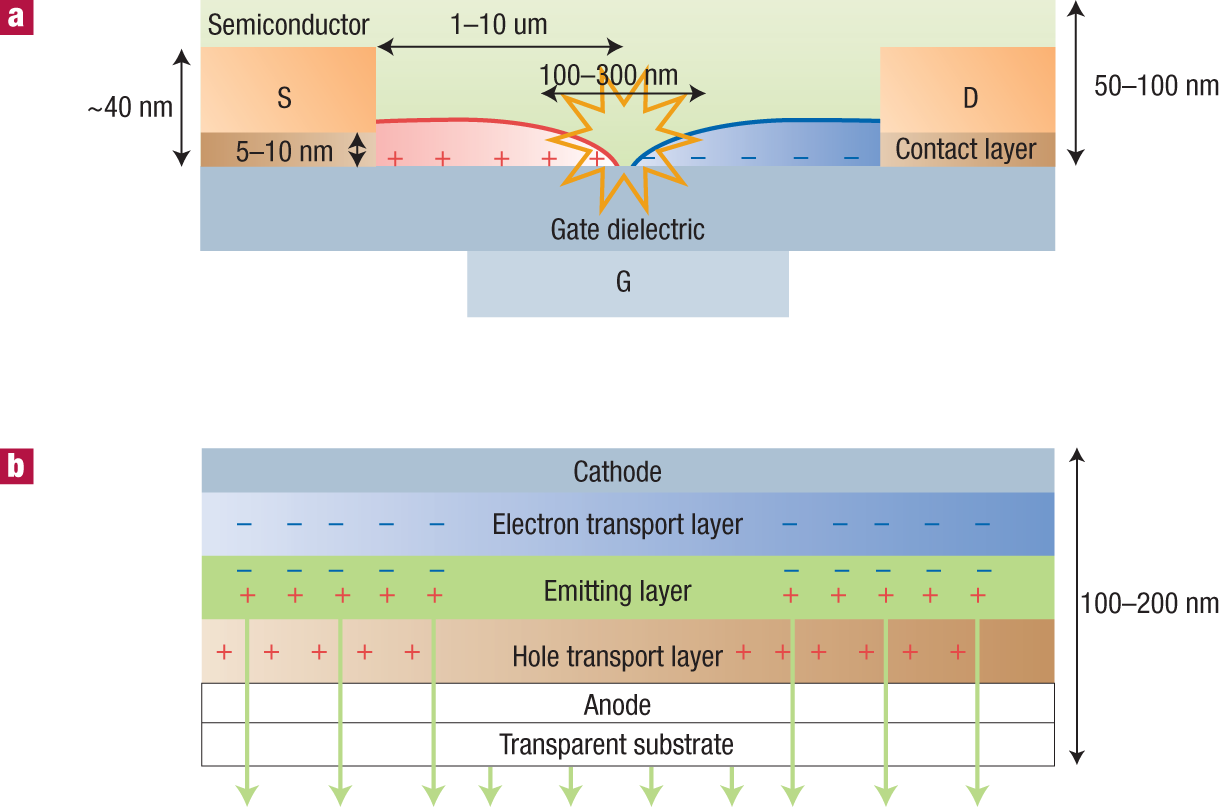
\includegraphics[width=0.8\textwidth]{fig_2}
  \caption{Schematic representation of \textsc{olet} and \textsc{oled}. (a) Horizontal charge transport in \textsc{olet}s. (b) Vertical charge transport in \textsc{oled}s. From \citet{Muccini}.}
  \label{fig:thinfilms}
 \end{center}
\end{figure}

The mobility of the charge carriers in this \textsc{olet} geometry can be up to four orders of magnitude higher than in the \textsc{oled}s. The \textsc{olet} has a potentially higher electroluminescence quantum efficiency, which is inherent to the device structure.

For \textsc{olet}s, the distance between the exciton formation region and the metal electrodes is much larger. Therefore they are less affected by electron-metal quenching. This effect is further reduced by the availability of a third electrode that balances electron and hole currents. These structural advantages make \textsc{olet}s more favourable for high-brightness electroluminescence and highly integrated devices. These advantages however do rely on the further development of organic materials.


A possible disadvantage for \textsc{olet} devices is the distance the charge carriers need to travel before recombining radiatively. For typical ambipolar \textsc{olet}s the distance is in the order of hundreds of nanometres or more, in \textsc{oled}s the distance the minority carriers travel are only in the order tens of nanometres. This requires stricter charge transport properties of \textsc{olet} materials.
